\subsection{Shell Sort}

Là một thuật toán sắp xếp dựa trên sắp xếp chèn (Insertion Sort), được 
đặt theo tên của người phát minh, Donald Shell. Thuật toán này cải tiến 
sắp xếp chèn bằng cách cho phép so sánh và hoán đổi các phần tử cách xa 
nhau trước khi thu hẹp khoảng cách lại. Điều này giúp giảm thiểu số lần 
hoán đổi và dịch chuyển các phần tử. Đây là một thuật toán không ổn định, 
phần tử bằng nhau có thể bị đổi chỗ do hoán đổi các nhóm cách xa nhau.

\subsubsection{Ý tưởng}

\begin{enumerate}
    \item Thay vì sắp xếp toàn bộ danh sách một cách tuần tự, Shell Sort 
    chia danh sách thành các danh sách con với khoảng cách giữa các phần 
    tử được xác định bởi một giá trị gọi là khoảng.
    \item Thuật toán sử dụng sắp xếp chèn để sắp xếp các phần tử trong 
    từng danh sách con này.
    \item Sau mỗi vòng lặp, khoảng cách được thu nhỏ dần, cuối cùng trở 
    về 1, lúc này danh sách được sắp xếp hoàn chỉnh.
\end{enumerate}

\subsubsection{Mã giả}

\begin{algorithm}[H]
    \caption{Shell Sort}
    \SetKwFunction{ShellSort}{ShellSort}
    \SetKwProg{Fn}{procedure}{:}{}
    \Fn{\ShellSort{a\KwSty{[ ]}, n}}{
        $gap \gets n / 2$ \tcp{Khởi tạo khoảng cách}
        \While{$gap > 0$}{
            \For{$i \gets gap$ \KwTo $n - 1$}{
                $temp \gets a[i],\ j \gets i$ \\
                
                \tcp{Dịch chuyển các phần tử lớn hơn temp lên một khoảng}
                \While{$j \geq gap$ \KwSty{and} $a[j - gap] > temp$}{
                    $a[j] \gets a[j - gap]$ \\
                    $j \gets j - gap$
                }
                $a[j] \gets temp$ \tcp{Đặt temp vào đúng vị trí}
            }
            $gap \gets gap / 2$ \tcp{Giảm khoảng cách}
        }
    }
\end{algorithm}

\subsubsection{Ví dụ}

Giả sử ta có mảng ban đầu với $n=5$ như sau:
\begin{center}
    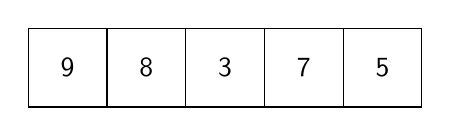
\begin{tikzpicture}[node distance=0cm, font=\sffamily, every node/.style={minimum width=1cm, minimum height=1cm, outer sep=0pt, anchor = west}, line join=miter, line cap=rect]
        \node[draw, fill=white] at (9, 0) {9};
        \node[draw, fill=white] at (10, 0) {8};
        \node[draw, fill=white] at (11, 0) {3};
        \node[draw, fill=white] at (12, 0) {7};
        \node[draw, fill=white] at (13, 0) {5};
    \end{tikzpicture}
\end{center}

Bắt đầu với $gap = 2$, thực hiện sắp xếp chèn với khoảng cách $gap$ 
cho từng phần tử từ vị trí $gap$ đến hết bên phải mảng.

\begin{center}
    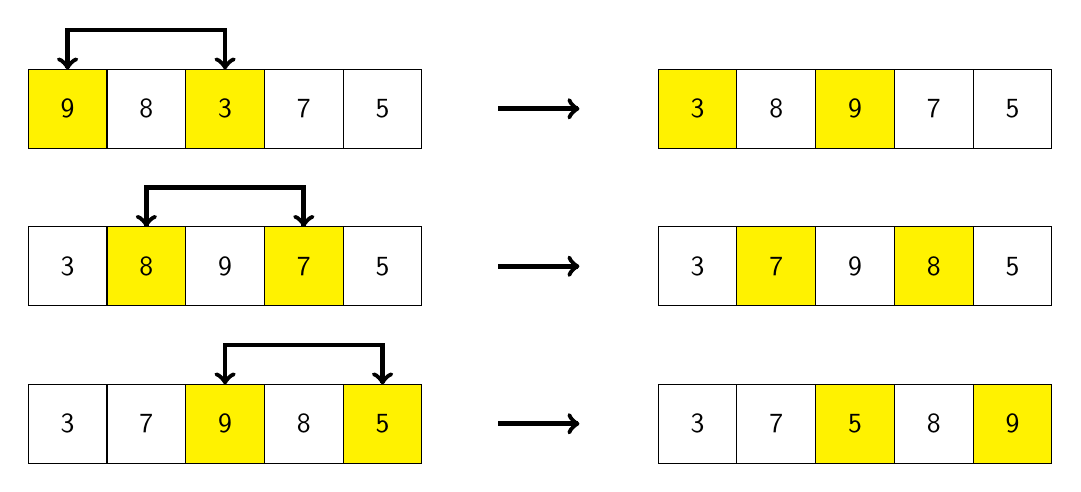
\begin{tikzpicture}[node distance=0cm, font=\sffamily, every node/.style={minimum width=1cm, minimum height=1cm, outer sep=0pt, anchor = west}, line join=miter, line cap=rect]
        % Substep 1
        \node[draw, fill=yellow] at (1, -3.5) {9};
        \node[draw, fill=white] at (2, -3.5) {8};
        \node[draw, fill=yellow] at (3, -3.5) {3};
        \node[draw, fill=white] at (4, -3.5) {7};
        \node[draw, fill=white] at (5, -3.5) {5};
        \draw[<-, line width=0.6mm, shorten <=0pt] (3.5, -3) -- (3.5, -2.5);
        \draw[line width=0.6mm] (3.5, -2.5) -- (1.5, -2.5);
        \draw[->, line width=0.6mm, shorten >=0pt] (1.5, -2.5) -- (1.5, -3);
        
        \draw[->, line width=0.6mm] (7, -3.5) -- (8, -3.5);
        
        \node[draw, fill=yellow] at (9, -3.5) {3};
        \node[draw, fill=white] at (10, -3.5) {8};
        \node[draw, fill=yellow] at (11, -3.5) {9};
        \node[draw, fill=white] at (12, -3.5) {7};
        \node[draw, fill=white] at (13, -3.5) {5};
        
        % Substep 2
        \node[draw, fill=white] at (1, -5.5) {3};
        \node[draw, fill=yellow] at (2, -5.5) {8};
        \node[draw, fill=white] at (3, -5.5) {9};
        \node[draw, fill=yellow] at (4, -5.5) {7};
        \node[draw, fill=white] at (5, -5.5) {5};
        \draw[<-, line width=0.6mm, shorten <=0pt] (4.5, -5) -- (4.5, -4.5);
        \draw[line width=0.6mm] (4.5, -4.5) -- (2.5, -4.5);
        \draw[->, line width=0.6mm, shorten >=0pt] (2.5, -4.5) -- (2.5, -5);
        
        \draw[->, line width=0.6mm] (7, -5.5) -- (8, -5.5);
        
        \node[draw, fill=white] at (9, -5.5) {3};
        \node[draw, fill=yellow] at (10, -5.5) {7};
        \node[draw, fill=white] at (11, -5.5) {9};
        \node[draw, fill=yellow] at (12, -5.5) {8};
        \node[draw, fill=white] at (13, -5.5) {5};
        
        % Substep 3
        \node[draw, fill=white] at (1, -7.5) {3};
        \node[draw, fill=white] at (2, -7.5) {7};
        \node[draw, fill=yellow] at (3, -7.5) {9};
        \node[draw, fill=white] at (4, -7.5) {8};
        \node[draw, fill=yellow] at (5, -7.5) {5};
        \draw[<-, line width=0.6mm, shorten <=0pt] (5.5, -7) -- (5.5, -6.5);
        \draw[line width=0.6mm] (5.5, -6.5) -- (3.5, -6.5);
        \draw[->, line width=0.6mm, shorten >=0pt] (3.5, -6.5) -- (3.5, -7);
        
        \draw[->, line width=0.6mm] (7, -7.5) -- (8, -7.5);
        
        \node[draw, fill=white] at (9, -7.5) {3};
        \node[draw, fill=white] at (10, -7.5) {7};
        \node[draw, fill=yellow] at (11, -7.5) {5};
        \node[draw, fill=white] at (12, -7.5) {8};
        \node[draw, fill=yellow] at (13, -7.5) {9};
    \end{tikzpicture}
\end{center}

Thực hiện tương tự với $gap = 1$, ta thu được mảng đã sắp xếp:

\begin{center}
    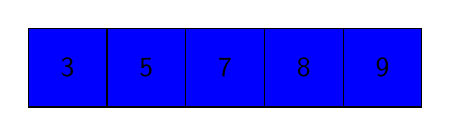
\begin{tikzpicture}[node distance=0cm, font=\sffamily, every node/.style={minimum width=1cm, minimum height=1cm, outer sep=0pt, anchor = west}, line join=miter, line cap=rect]
        \node[draw, fill=blue] at (9, 0) {3};
        \node[draw, fill=blue] at (10, 0) {5};
        \node[draw, fill=blue] at (11, 0) {7};
        \node[draw, fill=blue] at (12, 0) {8};
        \node[draw, fill=blue] at (13, 0) {9};
    \end{tikzpicture}
\end{center}

\subsubsection{Độ phức tạp thuật toán}

\begin{itemize}
    \item Độ phức tạp thời gian\\
    Hiệu suất của thuật toán Shell Sort phụ thuộc rất nhiều vào chuỗi 
    khoảng cách và thứ tự của mảng đầu vào (với chuỗi khoảng cách là tập 
    hợp tất cả các giá trị mà gap nhận trong quá trình thực hiện thuật 
    toán). Cụ thể:
    \begin{itemize}[label=$\circ$]
        \item Trường hợp tốt nhất: $O\left(n\log{n}\right)$, Khi mảng đầu vào 
        đã được sắp xếp hoàn toàn hoặc gần như sắp xếp và sử dụng một chuỗi 
        khoảng cách tối ưu (ví dụ: Knuth, Sedgewick,..). Vì khi mảng đã sắp 
        xếp, mỗi bước sắp xếp với khoảng cách gap chỉ cần thực hiện rất ít 
        phép so sánh và không cần hoán đổi. Còn chuỗi khoảng cách tối ưu đảm 
        bảo các phần tử được phân phối đều và nhanh chóng đưa mảng về trạng 
        thái sắp xếp hoàn chỉnh.

        \pagebreak

        \item Trường hợp xấu nhất: $O\left(n^2\right)$. Khi mảng đầu vào được 
        sắp xếp ngược và sử dụng chuỗi khoảng cách không tối ưu như $n,n/2,n/4,
        \ldots,1$, (giống trong mã giả nói trên). Trong trường hợp này, các 
        phần tử phải được di chuyển qua lại nhiều lần để đưa về đúng vị trí. 
        Đặc biệt, khi $gap = 1$, Shell Sort trở thành Insertion Sort, dẫn đến 
        hiệu suất tương tự là $O\left(n^2\right)$.
        \item Trường hợp trung bình: $O\left(n^{3/2}\right)$. Khi mảng đầu vào 
        có thứ tự ngẫu nhiên và sử dụng chuỗi khoảng cách phổ biến như $n,n/2,
        n/4,\ldots,1$. Trong trường hợp này, các phần tử không được phân phối 
        đều trong các lớp, dẫn đến việc cần thực hiện nhiều phép so sánh và 
        hoán đổi hơn. Đồng thời, với chuỗi khoảng cách không tối ưu, nhưng vẫn 
        đảm bảo hiệu suất tốt hơn so với Insertion Sort với độ phức tạp theo 
        thời gian trung bình là $O\left(n^2\right)$.
    \end{itemize}
    Lưu ý: Chuỗi khoảng cách là tập hợp tất cả các giá trị mà $gap$ nhận 
    trong quá trình thực hiện thuật toán.
    
    \item Độ phức tạp không gian: $O\left(1\right)$, vì Shell Sort là một 
    thuật toán in-place, nghĩa là nó không sử dụng bất kỳ cấu trúc dữ liệu 
    phụ nào ngoài một số biến tạm thời. Toàn bộ việc sắp xếp được thực hiện 
    trực tiếp trên mảng đầu vào. 
\end{itemize}